\section{System Overview}
\label{s:overview}
\begin{figure}[!t]
\centering
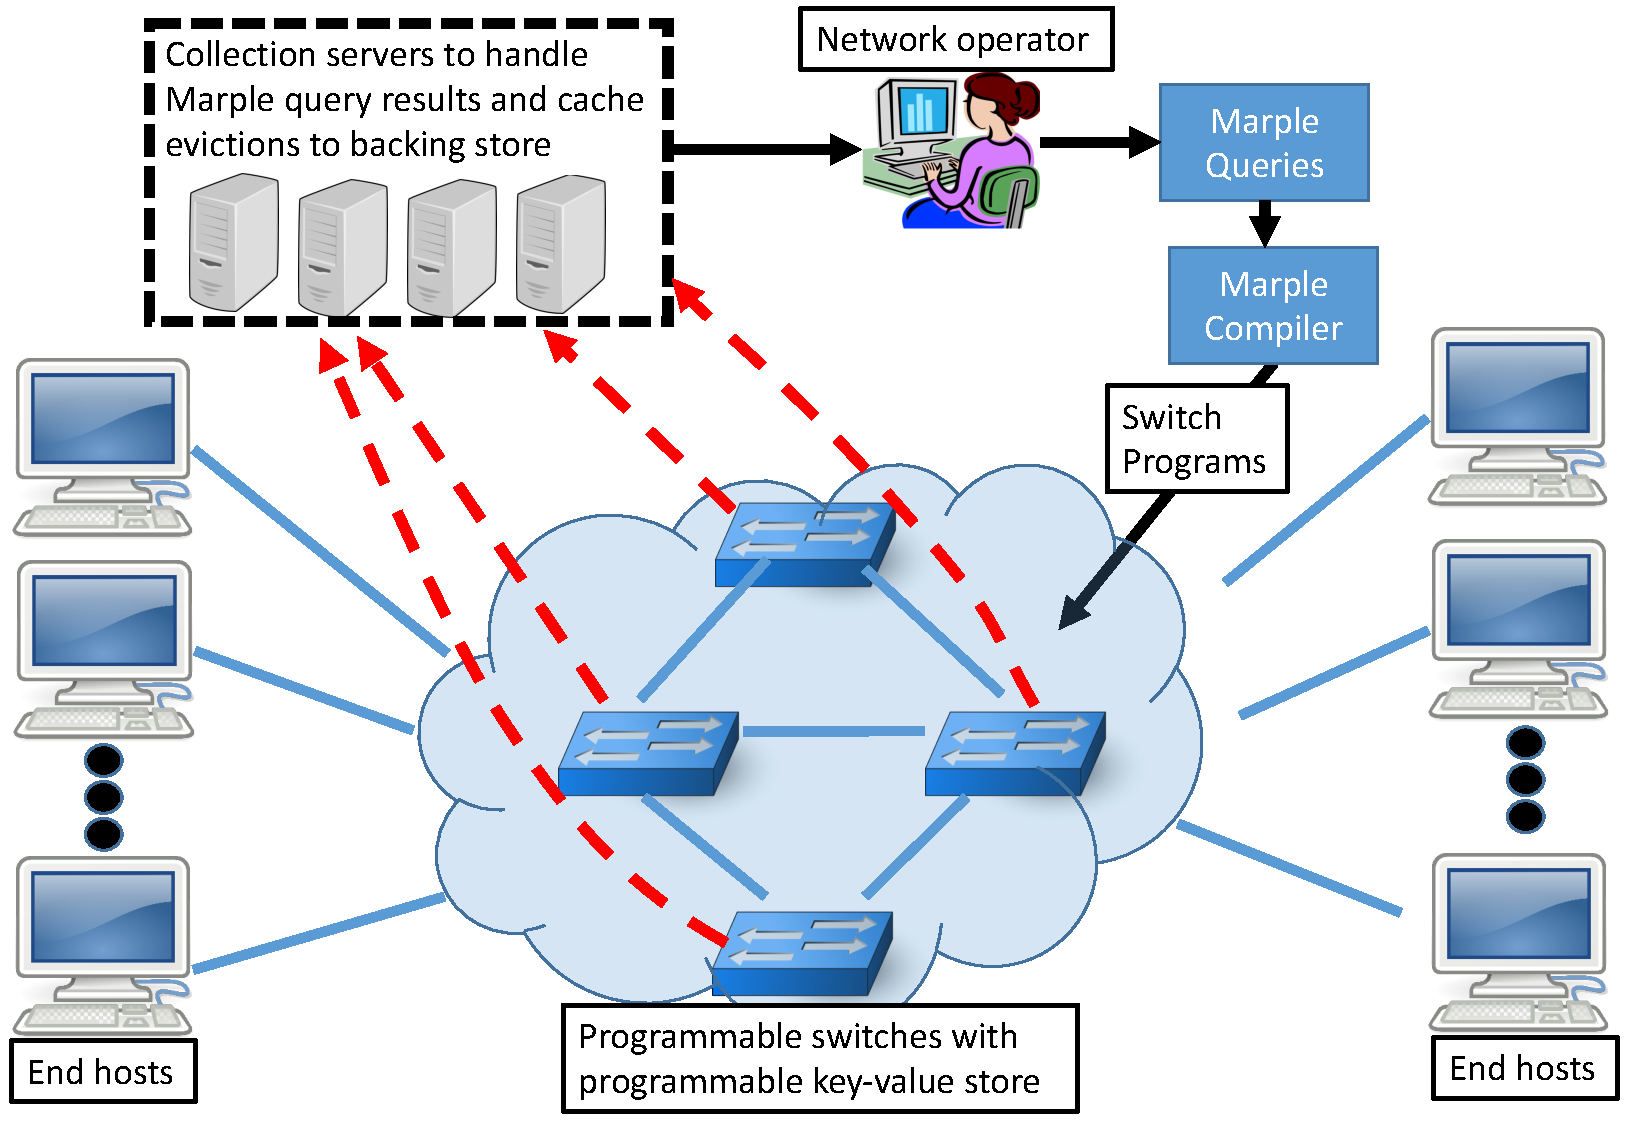
\includegraphics[width=0.7\columnwidth]{pq_overview.pdf}
\caption{An operator issues a \TheSystem query, which is compiled into
switch programs for programmable switches augmented with our
key-value store. Streamed results from this query are available in
collection servers that also contain the backing store for the key-value
store.}
\label{fig:overview}
\end{figure}

A performance query language provides a convenient abstraction to ask
network-performance-related questions. But how should the underlying monitoring
be implemented?

A naive implementation would collect and store every packet's metadata
from the network in a logically centralized database, and issue performance
queries against this database. %% Some research efforts advocate a
%% similar approach to run arbitrary queries over network
%% data~\cite{netsight}. However, the approach is impractical for large
%% networks. 
Modern scale-out data-processing systems support hundreds of thousands of
operations per second per core~\cite{kafka_benchmark, redis_benchmark,
  memcached_benchmark, redis_vs_memcached, redis_vs_memcached_update}. At such
rates, the compute resources required to process a multi-Tb/s stream from each
switch (tens of millions of packets/second) make this implementation
unviable.

Our approach is to leverage high-speed programmable switches~\cite{rmt, xpliant,
  tofino, flexpipe} as first-class citizens in network monitoring---processing
packets at line-rate {\em and} providing accurate query results.
%% While this approach has been adopted by some
%% research prototypes~\cite{netsight} and allows operators to run arbitrary
%% queries on the collected data, it is unlikely to scale to larger networks
%% because of the sheer amount of information that is collected.\footnote{Sampling
%%   is a solution, but the loss in accuracy from sampling can be arbitrarily large
%%   depending on the query. Our work focuses on queries with no loss in accuracy.}
%% Approaches that collect packets and then analyze them on collection servers
%% implicitly take the view that any reasonable computation on packet data must
%% happen on end-hosts that can be programmed to execute an operator's queries.
%% The emergence of high-speed programmable switches~\cite{rmt, xpliant, tofino,
%% flexpipe} lets us view switches as first-class citizens in the execution of
%% such queries.
%% Instead of passively streaming every packet to a measurement database,
%% %% active versus passive point: removed
The instructions on these switches can aggregate packets into per-flow counters
({\ct groupby}), transform packet fields ({\ct map}), stream only user-specified
packets ({\ct filter}), or merge packets that satisfy two previous queries ({\ct
  zip}). Flexible filtering and aggregation on a switch drastically reduces the
amount of data that is materialized as the result of a query, which makes
handling the query results using standard data-processing systems much more
feasible.

%TODO: State somewhere that we don't need a zillion open-flow rules, only one default action.
Of the four language constructs, three of them, \ie {\ct map}, {\ct filter}, and
{\ct zip}, are stateless: they operate on packet fields and do not modify switch
state. Such stateless manipulations are already supported on emerging
programmable switches~\cite{rmt, xpliant, flexpipe, tofino}.

On the other hand, the {\ct groupby} construct should maintain state on switches.
%% It is the most powerful of our language constructs and captures the kind of
%% complex processing typically seen at end hosts.
Stateful manipulation on a switch is challenging because the time budget to
update state before the next packet arrives can be as low as a nanosecond on
high-end switches~\cite{domino_sigcomm}.  Further, the switch may need to
maintain a total amount of state proportional to the number of flows, which may
grow unbounded with time.

We solve both challenges through a novel programmable key-value store in
hardware, where the keys represents aggregation fields (\eg flows) and values
represent the state being aggregated across packets. Our key-value store has a
`split' design: a small on-chip cache on the switch processes packets at line
rate, while a large off-chip backing store allows us to scale to a large number
of flows.

\Fig{overview} provides an overview of how \TheSystem may be used in a
monitoring system by a network operator. An operator writes a \TheSystem query,
either to implement a long-running monitor for a statistic (\eg TCP timeouts),
or to troubleshoot a specific problem at hand. The query is compiled into a
switch program that runs on the network's programmable switches, augmented with
our key-value store. The switch streams tuples and key-value pairs out to
collection servers, where the operator can retrieve query results.
